\documentclass[unicode,11pt,a4paper,oneside,numbers=endperiod,openany]{scrartcl}

\usepackage{xcolor}
\usepackage{listings}
\usepackage{amsmath}

\lstnewenvironment{grayverbatim}{
  \lstset{backgroundcolor=\color{gray!10}, % Adjust the shade of gray as desired
          frame=single,
          framerule=0pt,
          basicstyle=\ttfamily,
          breaklines=true,
          columns=fullflexible}
}{}

\lstnewenvironment{cppverbatim}{
  \lstset{language=C++, % Set the language to C++
          backgroundcolor=\color{gray!10}, % Adjust the shade of gray as desired
          frame=single,
          framerule=0pt,
          basicstyle=\ttfamily,
          keywordstyle=\color{blue}, % Set the color for keywords
          commentstyle=\color{green!50!black}, % Set the color for comments
          stringstyle=\color{red}, % Set the color for strings
          breaklines=true,
          showstringspaces=false, % Don't show spaces within strings
          columns=fullflexible}
}{}

\lstnewenvironment{pythonverbatim}{
    \lstset{language=Python, % Set the language to Python
            backgroundcolor=\color{gray!10}, % Adjust the shade of gray as desired
            frame=single,
            framerule=0pt,
            basicstyle=\ttfamily,
            keywordstyle=\color{blue}, % Set the color for keywords
            commentstyle=\color{green!50!black}, % Set the color for comments
            stringstyle=\color{red}, % Set the color for strings
            breaklines=true,
            showstringspaces=false, % Don't show spaces within strings
            columns=fullflexible}
}{}

\usepackage{ifthen}
\usepackage[utf8]{inputenc}
\usepackage{graphics}
\usepackage{graphicx}
\usepackage{hyperref}

\pagestyle{plain}
\voffset -5mm
\oddsidemargin  0mm
\evensidemargin -11mm
\marginparwidth 2cm
\marginparsep 0pt
\topmargin 0mm
\headheight 0pt
\headsep 0pt
\topskip 0pt        
\textheight 255mm
\textwidth 165mm

\newcommand{\duedate} {}
\newcommand{\setduedate}[1]{%
\renewcommand\duedate {Due date:~ #1}}
\newcommand\isassignment {false}
\newcommand{\setassignment}{\renewcommand\isassignment {true}}
\newcommand{\ifassignment}[1]{\ifthenelse{\boolean{\isassignment}}{#1}{}}
\newcommand{\ifnotassignment}[1]{\ifthenelse{\boolean{\isassignment}}{}{#1}}

\newcommand{\assignmentpolicy}{
\begin{table}[h]
\begin{center}
\scalebox{0.8} {%
\begin{tabular}{|p{0.02cm}p{16cm}|}
\hline
&\\
\multicolumn{2}{|c|}{\Large\textbf{HPC Lab for CSE 2024 ---  Submission Instructions}}\\
\multicolumn{2}{|c|}{\large\textbf{(Please, notice that following instructions are mandatory: }}\\
\multicolumn{2}{|c|}{\large\textbf{submissions that don't comply with, won't be considered)}}\\
&\\
\textbullet & Assignments must be submitted to \href{https://moodle-app2.let.ethz.ch/course/view.php?id=22516}{Moodle} (i.e. in electronic format).\\
\textbullet & Provide both executable package and sources (e.g. C/C++ files, Matlab). 
If you are using libraries, please add them in the file. Sources must be organized in directories called:\\
\multicolumn{2}{|c|}{\textit{Project\_number\_lastname\_firstname}}\\
& and  the  file must be called:\\
\multicolumn{2}{|c|}{\textit{project\_number\_lastname\_firstname.zip}}\\
\multicolumn{2}{|c|}{\textit{project\_number\_lastname\_firstname.pdf}}\\
\textbullet &  The TAs will grade your project by reviewing your project write-up, and looking at the implementation 
                 you attempted, and benchmarking your code's performance.\\

\textbullet & You are allowed to discuss all questions with anyone you like; however: (i) your submission must list anyone you discussed problems with and (ii) you must write up your submission independently.\\
\hline
\end{tabular}
}
\end{center}
\end{table}
}
\newcommand{\punkte}[1]{\hspace{1ex}\emph{\mdseries\hfill(#1~\ifcase#1{Points}\or{Points}\else{Points}\fi)}}


\newcommand\serieheader[6]{
\thispagestyle{empty}%
\begin{flushleft}

\includegraphics[width=0.4\textwidth]{ETHlogo_13}
\end{flushleft}
  \noindent%
  {\large\ignorespaces{\textbf{#1}}\hspace{\fill}\ignorespaces{ \textbf{#2}}}\\ \\%
  {\large\ignorespaces #3 \hspace{\fill}\ignorespaces #4}\\
  \noindent%
  \bigskip
  \hrule\par\bigskip\noindent%
  \bigskip {\ignorespaces {\Large{\textbf{#5}}}
  \hspace{\fill}\ignorespaces \large \ifthenelse{\boolean{\isassignment}}{\duedate}{#6}}
  \hrule\par\bigskip\noindent%  \linebreak
 }

\makeatletter
\def\enumerateMod{\ifnum \@enumdepth >3 \@toodeep\else
      \advance\@enumdepth \@ne
      \edef\@enumctr{enum\romannumeral\the\@enumdepth}\list
      {\csname label\@enumctr\endcsname}{\usecounter
        {\@enumctr}%%%? the following differs from "enumerate"
	\topsep0pt%
	\partopsep0pt%
	\itemsep0pt%
	\def\makelabel##1{\hss\llap{##1}}}\fi}
\let\endenumerateMod =\endlist
\makeatother




\usepackage{textcomp}






\begin{document}


\setassignment
\setduedate{Monday 13 May 2024, 23:59 (midnight).}

\serieheader{High-Performance Computing Lab for CSE}{2024}
            {Student: CARLA JUDITH LOPEZ ZURITA}
            {Discussed with: FULL NAME}{Solution for Project 5}{}
\newline

\assignmentpolicy


Project 5 is about continuing the work on the parallel solution of a nonlinear
PDE using MPI and learning about Python for High-Performance Computing.

\section{Parallel Space Solution of a nonlinear PDE using MPI
         [in total 60 points]}
Following the steps of Project 3, we will parallelize the solution of the
diffusion equation using MPI. We will also implement parallel I/O to write
the solution to disk. We will then evaluate the strong and weak scaling of
our parallel implementation.
\subsection{Initialize/finalize MPI and welcome message [5 Points]}
The code should initialize MPI, get the number of processes, and print a welcome
message. After adding the header for the library, only a few lines of code were changed to initialize MPI and print the welcome message. The following code snippet shows the changes made to the code:
\begin{cppverbatim}
std::cout << "version   :: C++ MPI" << std::endl;
std::cout << "processes :: " << size << std::endl;
\end{cppverbatim}
As well as finalizing MPI at the end of the code and adding relevant print
conditions for only the master thread.
\subsection{Domain decomposition [10 Points]}

On the \texttt{data.cpp} file, some changes were added to the SubDomain struct
very similar to those in Project 3.  The
strategy implemented is based in determining automatically the number of
subdomains in the $x$ and $y$ dimensions using the \texttt{MPI\_Dims\_create}
function. The following code snippet shows the changes made to the code:
\begin{cppverbatim}
int dims[2] = {0, 0};
MPI_Dims_create(mpi_size, 2, dims);
ndomy = dims[0];
ndomx = dims[1];
\end{cppverbatim}
We also added the \texttt{MPI\_Cart\_create} function to create the Cartesian as
well as the \texttt{MPI\_Cart\_coords} function to determine the coordinates of
each process and the \texttt{MPI\_Cart\_shift} function to determine the neighbors.
We also added some conditions to adjust the
cases for when a dimension is not divisible by the number of processes.

TODO: Discuss why this method was selected and analyze its implications on the performance of the application.
% Consider aspects such as load balancing, communication overhead, and
% computational efficiency in your analysis.
% Hint: Consider the number of data that must be communicated by a generic process with its neighbors.
% See the short discussion in [1, Sec. 10.4.1]
\subsection{Linear algebra kernels [5 Points]}
Next, we parallelized the relevant linear algebra kernels in  \texttt{hpc\_XXX}
in \texttt{linalg.cpp} using MPI. Not all funcitons needed to be modified, only
the ones that required communication between processes, such as \texttt{hpc\_dot}
and \texttt{hpc\_norm2}. Both follow the same pattern of using the
\texttt{MPI\_Allreduce}. The code snippet below shows the changes made to the
\texttt{hpc\_dot} function:
\begin{cppverbatim}
// computes the inner product of x and y
// x and y are vectors on length N
double hpc_dot(Field const& x, Field const& y) {
    double global_result;
    double local_result = 0.0;
    int N = y.length();
    // compute local result
    for (int i = 0; i < N; i++) {
        local_result += x[i] * y[i];
    }
    MPI_Allreduce(&local_result, &global_result, 1, MPI_DOUBLE, MPI_SUM, MPI_COMM_WORLD);
    return global_result;
}
\end{cppverbatim}
The rest of the functions were left unchanged.
\subsection{The diffusion stencil: Ghost cells exchange [10 Points]}
The next step was to implement the exchange of ghost cells between neighboring
processes. This was done by adding the \texttt{MPI\_Isend} and \texttt{MPI\_Irecv} functions to the
\texttt{diffusion} function in \texttt{operators.cpp}. 
This requeired following a series of steps.
First, we needed to fill the send buffer with the values of the ghost cells.
This was a bit tricky becase the indices needed to be inverted. 
\begin{cppverbatim}
// Fill buffers
for (int k = 0; k < nx; k++)
{
    // The indices needed to be inverted
    buffN[k] = s_new(k,jend);
    buffS[k] = s_new(k,0);
}
for (int k = 0; k < ny; k++)
{
    buffE[k] = s_new(iend,k);
    buffW[k] = s_new(0,k);
}
\end{cppverbatim}
Then, we needed to send the values and receive the values from the neighbours
using non-blocking point-to-pointcommunication. A custom data type was not
needed since we were sending contiguous data. The following code snippet shows
the changes made to the code:
\begin{cppverbatim}
MPI_Request request[8];
int tag1 = 1, tag2 = 2, tag3 = 3, tag4 = 4;
int count = 0;
    
// SEND
//  to top
MPI_Isend(&buffN[0], nx, MPI_DOUBLE, domain.neighbour_north, tag1, domain.comm_cart, &request[count++]);
//  to bottom
MPI_Isend(&buffS[0], nx, MPI_DOUBLE, domain.neighbour_south, tag2, domain.comm_cart, &request[count++]);
//  to right
MPI_Isend(&buffE[0], ny, MPI_DOUBLE, domain.neighbour_east, tag3, domain.comm_cart, &request[count++]);
//  to left
MPI_Isend(&buffW[0], ny, MPI_DOUBLE, domain.neighbour_west, tag4, domain.comm_cart, &request[count++]);

// RECEIVE
// from top
MPI_Irecv(&bndN[0], nx, MPI_DOUBLE, domain.neighbour_north, tag2, domain.comm_cart, &request[count++]);
// from bottom
MPI_Irecv(&bndS[0], nx, MPI_DOUBLE, domain.neighbour_south, tag1, domain.comm_cart, &request[count++]);
// from right
MPI_Irecv(&bndE[0], ny, MPI_DOUBLE, domain.neighbour_east, tag4, domain.comm_cart, &request[count++]);
// from left
MPI_Irecv(&bndW[0], ny, MPI_DOUBLE, domain.neighbour_west, tag3, domain.comm_cart, &request[count++]);
\end{cppverbatim}
Finally, we added a \texttt{MPI\_Waitall} function to wait for all the communications to finish.

\subsection{Implement parallel I/O [10 Points]}
Finally, we implemented parallel I/O to write the solution to disk. We used as
base the code provided in the assignment. The code in \texttt{main.cpp} was
modified to use a new version of \texttt{write\_binary} that uses MPI I/O. The
function is based on the \texttt{MPI\_File\_write\_at\_all} function, calling on
each subdomain to write its own data. One of the main changes was to change the
order to \texttt{MPI\_ORDER\_FORTRAN} to match the order of the data in the
file.
An example of the output image is shown in Figure \ref{fig:output}, which was
generated using $2048 \times 2048$ grid points and 32 processes.
\begin{figure}[h]
    \centering
    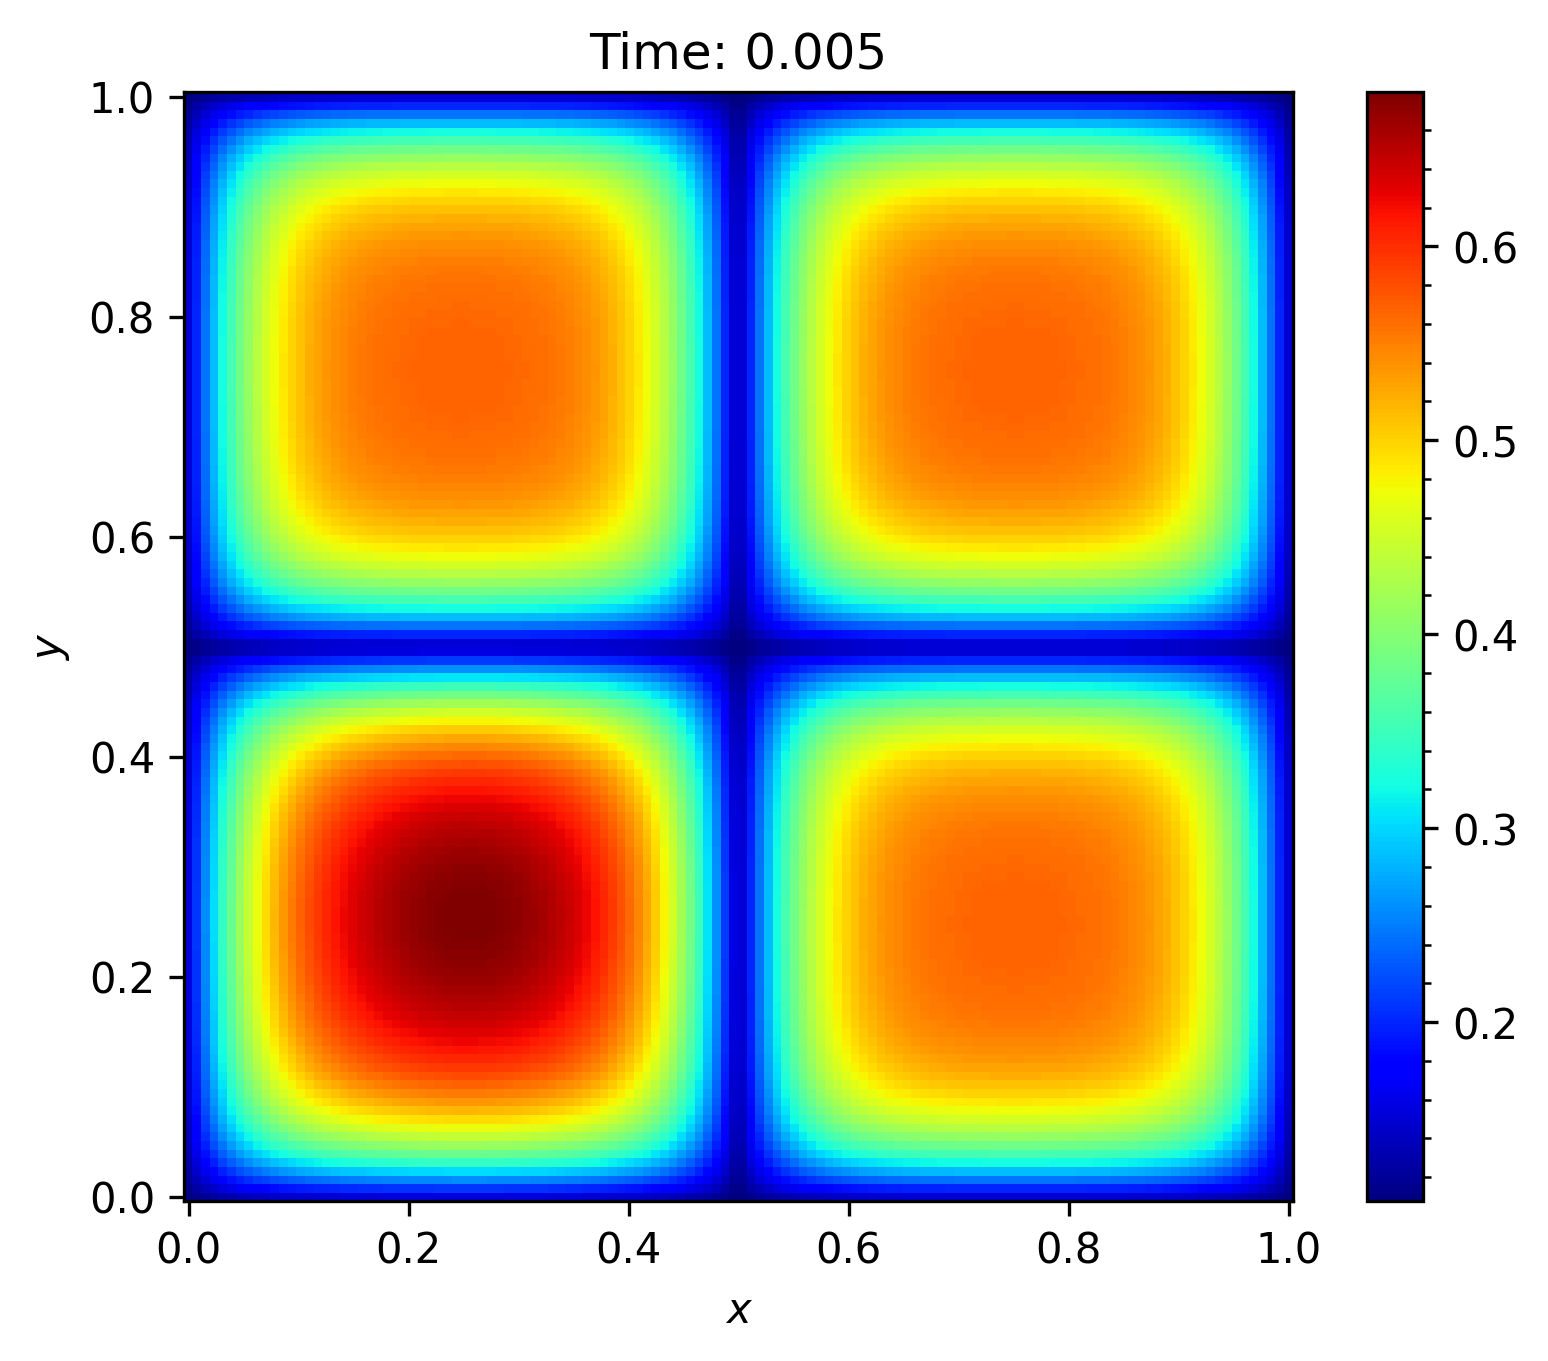
\includegraphics[width=0.5\textwidth]{../mini_app_mpi/output.png}
    \caption{Example of the output image using $2048 \times 2048$ grid points and 32 processes.}
    \label{fig:output}
\end{figure}


\subsection{Strong scaling [10 Points]}
Each configuration was run fifty times in order to get a more representative
time. The distribution of the data is shown in Figure \ref{fig:data}. Warm up
runs were included in the data, since they didn't seem to fall outside the distribution.
\begin{figure}[h!]
    \centering
    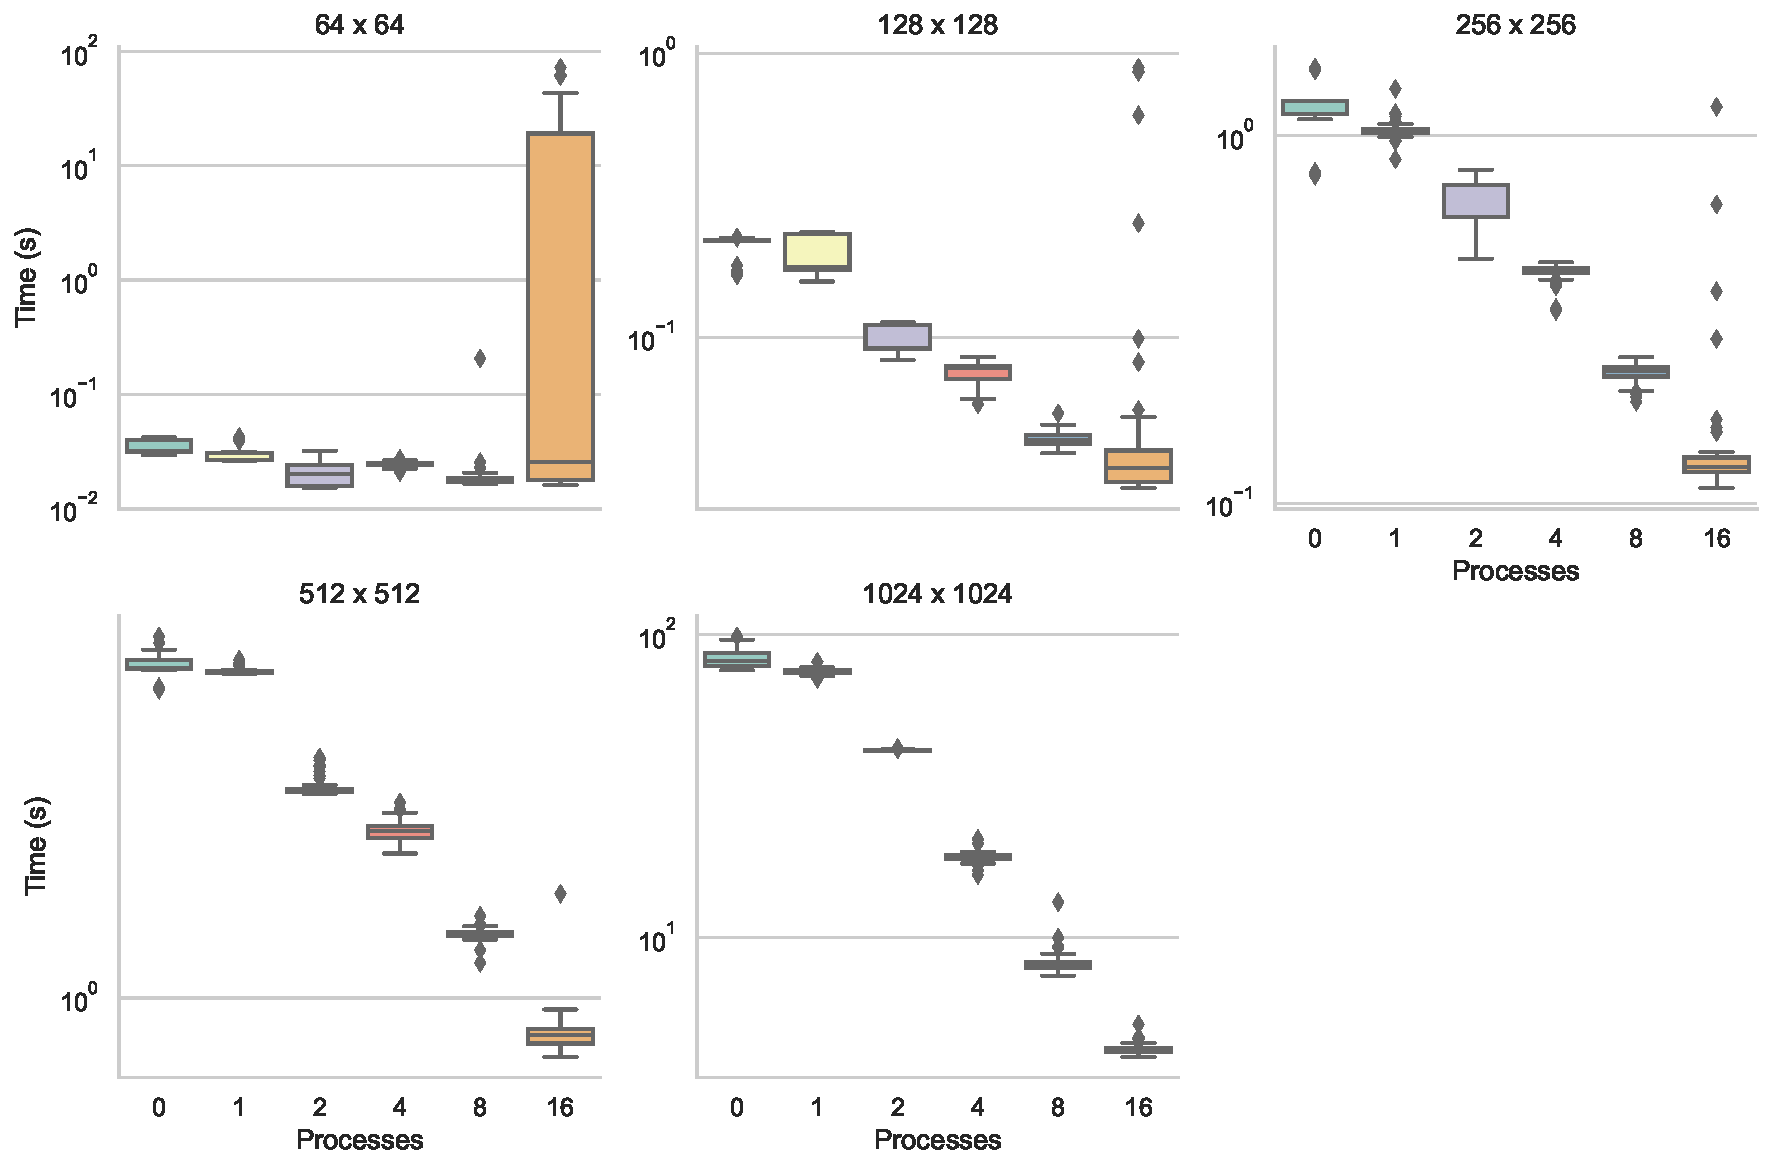
\includegraphics[width=\textwidth]{../mini_app_mpi/data_var_strong.pdf}
    \caption{Data distribution of the runtimes for different configurations of
    the parallel diffusion equation solver. Zero processes indicates the serial version.}
    \label{fig:data}
\end{figure}
We can see that for low number of processes, the data is not very spread out,
but as the number of processes increases, the distribution is also wider,
specially for a low number of grid points. 
This is expected since the
communication overhead increases with the number of processes, and is specially
noticeable for a low number of grid points where parallelization is not as
effective. We can see that for a high number of grid points, the distribution
is consistent. 
As serial version, I used the version of the code that doesn't use MPI, and is
shown in the plot using the label $0$ processes. 
Interestingly, we can see some cases
where the parallel version using one thread is faster than the serial version.
Both versions
were both compiled using the same flags but different compilers, namely \texttt{c++} for
the serial version and \texttt{mpicxx} for the parallel version. I am not sure if this
affects the results.
The results of
the strong scaling are shown in the Figure \ref{fig:strong}. The data point used
to generate the plot is the median of the fifty runs.
\begin{figure}[h!]
    \centering
    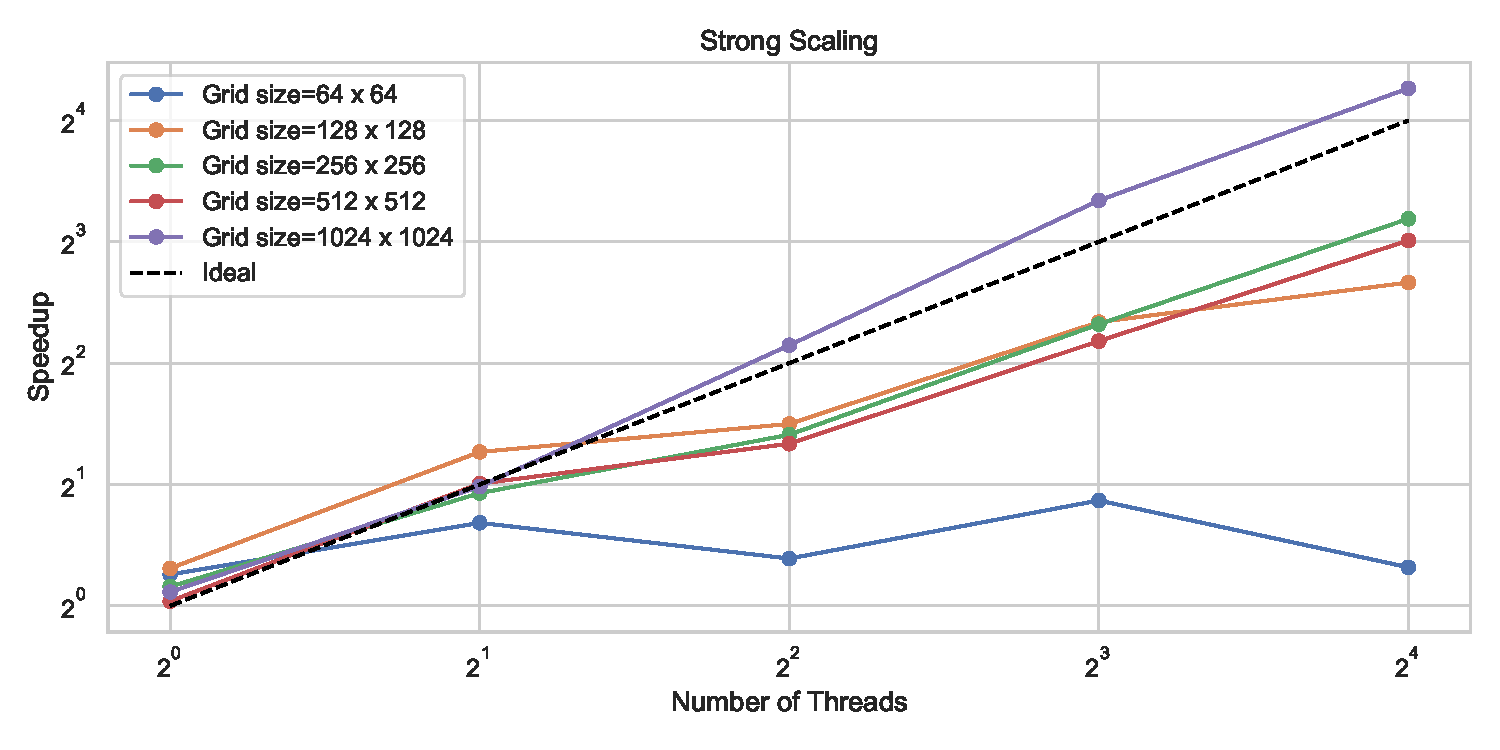
\includegraphics[width=\textwidth]{../mini_app_mpi/strong_scaling_plot.pdf}
    \caption{Strong scaling of the parallel diffusion equation solver.}
    \label{fig:strong}
\end{figure}
We can see consistent speedup for a high number of grid points, but the speedup
is not as good for a low number of grid points. 
The case of grid size $64 \times 64$ is the one with the worst speedup, showing almost no speedup at all.
This is expected due to the communication overhead as discussed previously. 
The case of grid size $1024
\times 1024$ is the one with the best speedup, showing beyond ideal speedup,
which could be a result of the times taken from the serial version being slower
due to some unknown reason. 

\subsection{Weak scaling [10 Points]}
Again the data was run fifty times for each configuration. The distribution of
the data is shown in Figure \ref{fig:data_weak}. Warm up runs were included in
the data, since they didn't seem to fall outside the distribution.
\begin{figure}[h!]
    \centering
    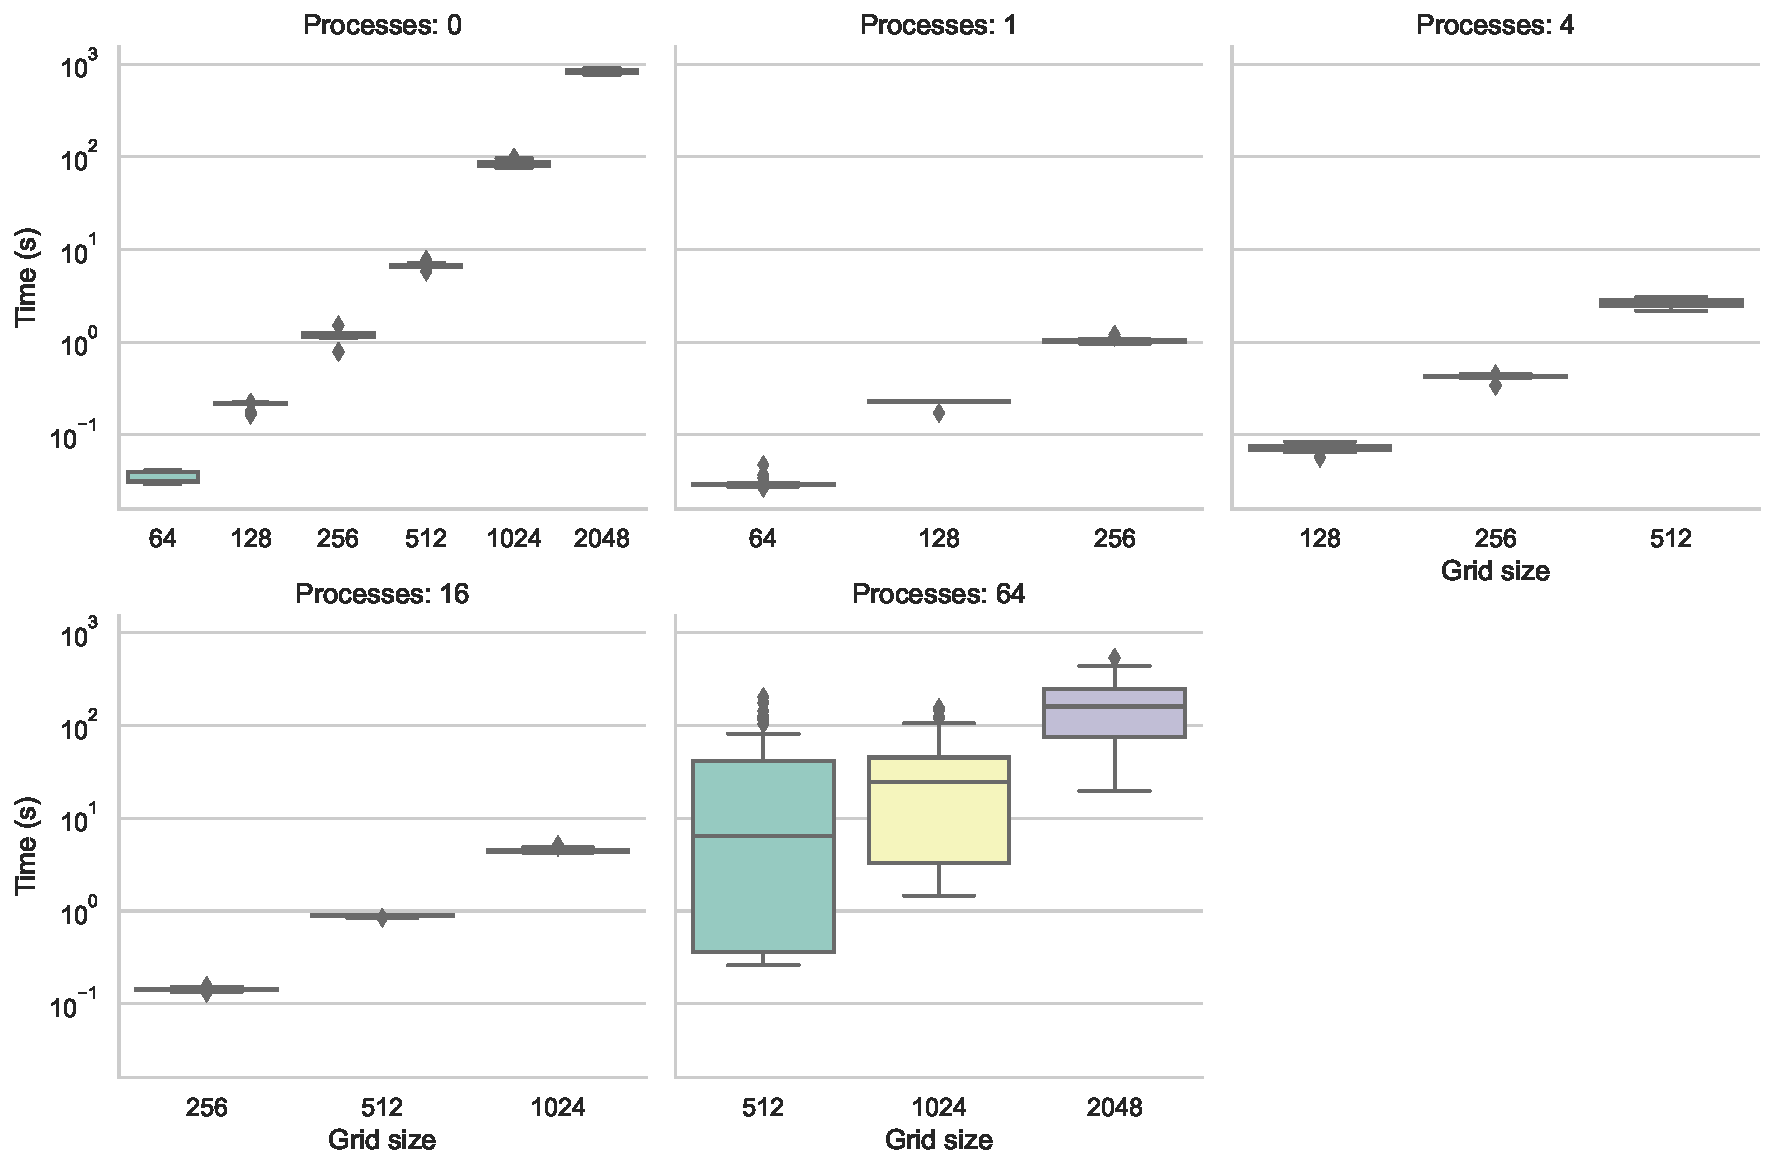
\includegraphics[width=\textwidth]{../mini_app_mpi/data_var_weak.pdf}
    \caption{Data distribution of the runtimes for different configurations of
    the parallel diffusion equation solver.}
    \label{fig:data_weak}
\end{figure}
This plot is inverted with respect to the strong scaling data visualization,
since the needs for the weak scaling require different configurations.
We can see that for each number of processes, the data increases as the number
of grid points increases. This is expected since the computation time increases
with the number of grid points. The data is not very spread out, which is
a good indication of low variability in runtimes, except for the case of $64$
processes, where the distribution is significantly wider. This is expected since
it correlates with the overhead in communication.

The results of the weak scaling are shown in the Figure \ref{fig:weak}.
\begin{figure}[h!]
    \centering
    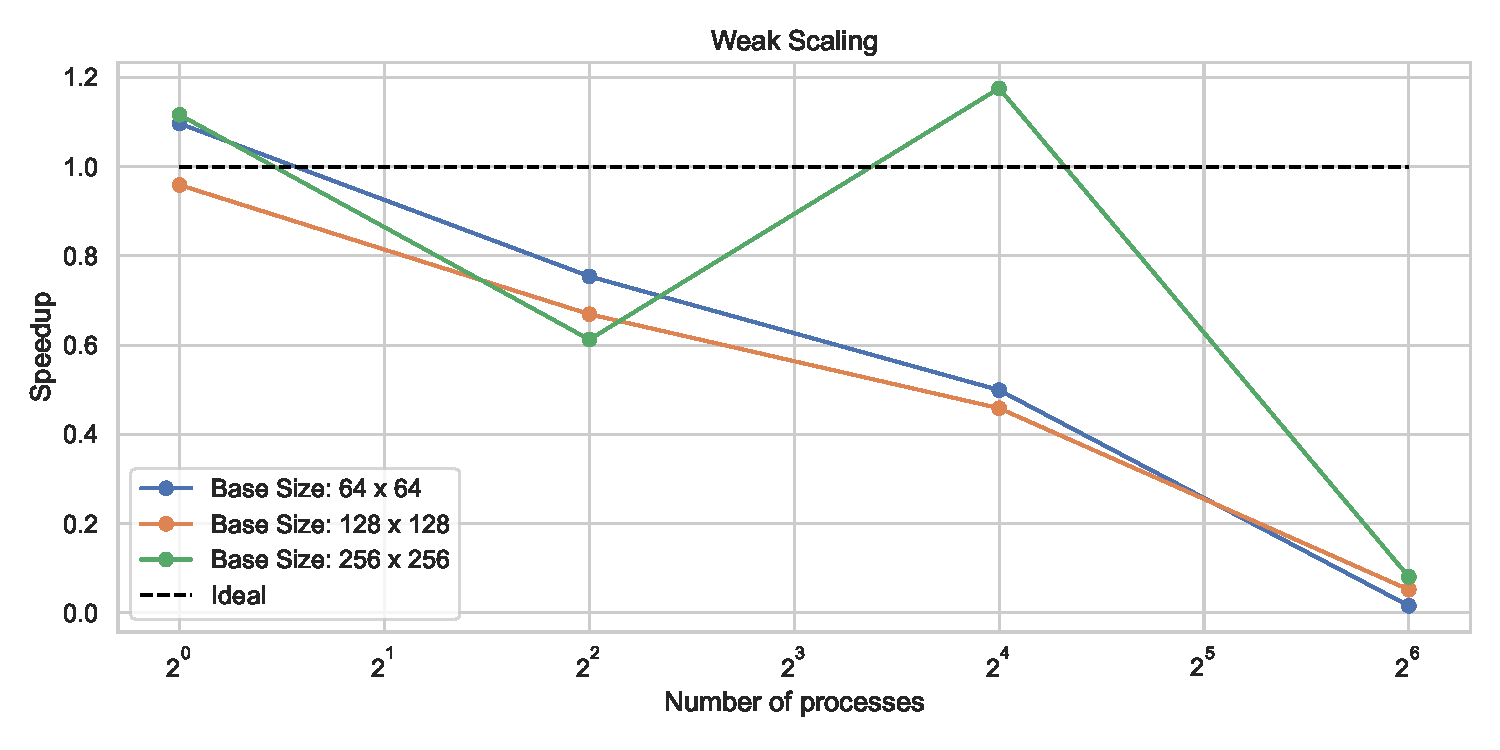
\includegraphics[width=\textwidth]{../mini_app_mpi/weak_scaling_plot.pdf}
    \caption{Weak scaling of the parallel diffusion equation solver.}
    \label{fig:weak}
\end{figure}
It shows a somewhat expected result, except for the case of $256 \times 256$
grid points as base case, where the speedup seems to be better than expected.
The behaviour of the rest of the data points is consistent with the expected
results, showing a decrease in speedup as the number of processes increases,
even though the number of grid points also increases. Interestingly, the
decrease in speedup is consistent for all the cases of starting grid points,
which tells us that for this condigurations, using 32 processes is not good
practice. Combined with the strong scaling results, we can see that the best
number of processes to use is 16, since it shows a good speedup for all the
cases. I am not sure why the speedup for the case of $256 \times 256$ grid
ppoints using 16 processes is better than expected, but it could be related to hardware being
optimal at that number of processes and grid points.

\subsection{Bonus [20 Points]: Overlapping computation/computation details}


\section{Python for High-Performance Computing [in total 40 points]}
In this section of the project, we will learn about MPI for Python and use it
to parallelize the computation of the Mandelbrot set. We will use a
manager-worker
pattern to distribute the computation of the Mandelbrot set among the workers.

Every python code using mpi4py is initialized with the following lines:
\begin{pythonverbatim}
from mpi4py import MPI

comm = MPI.COMM_WORLD
size = comm.Get_size()
rank = comm.Get_rank()
proc = MPI.Get_processor_name()
\end{pythonverbatim}
\subsection{Sum of ranks: MPI collectives [5 Points]}

Using MPI for Python's collective communication methods, we wrote a script that
computes the sum of all ranks. 
This was done using the pickle-based communication of generic Python objects as
well as the fast, near C-speed, direct array data communication of
buffer-provider objects.
The following code snippets show the changes made to the code using lower case functions:
\begin{pythonverbatim}
global_sum = comm.gather(rank)
if rank==0:
print(f"Sum: {sum(global_sum)}")
\end{pythonverbatim}
as well as using the uppercase functions:
\begin{pythonverbatim}
rank_array = np.array(rank, dtype=np.int32)
total_sum = np.zeros(1, dtype=np.int32)
comm.Allreduce(rank_array, total_sum, op=MPI.SUM)

if rank==0:
print(f"Sum: {sum(total_sum)}")
\end{pythonverbatim}
As the description of the assignment suggests, the uppercase functions are more
efficient and also need to use arrays to store the data, otherwise the code will not work.
Running the code with \texttt{salloc -n 8 --nodes=4 --ntasks-per-node=2}, the
output for both was:
\begin{grayverbatim}
Sum: 28
\end{grayverbatim}
Both methods worked as expected (7+6+5+4+2+3+1+0).

\subsection{Ghost cell exchange between neighboring processes [5 Points]}
Now, we implemented the exchange of ghost cells between neighboring processes
using MPI for Python.
This replicates the same functionality as in the C++ code, done in project 4.
First, we need to determine the number of subsections in the $x$ and $y$
dimensions, depending on the number of processes. This was done using the
\texttt{Compute\_dims} function. Then, we created a periodic Cartesian grid using the
\texttt{Create\_cart} function. We also used the \texttt{Shift} function to
determine the coordinates of the neighbors. The following code snippet shows
the implemented code:
\begin{pythonverbatim}
# Create dims depending on number of ranks
dims = [0, 0]
dims = MPI.Compute_dims(size, dims)

# Create cartesian grid
periods = [True, True]
cart2d = comm.Create_cart(dims, periods, reorder=False)
coords = cart2d.Get_coords(rank)

# Get coordinates of the neighbours
west, east = cart2d.Shift(direction=1, disp=1)
north, south = cart2d.Shift(direction=0, disp=1)
\end{pythonverbatim}
After filling a numpy array with the value of the rank, we excahnge the ghost
cells with the neighbors using the \texttt{Sendrecv} function. 
I decideded to use this function instead of the \texttt{sendrecv} for python
objects, since it is more efficient and made sense with the description of the
project since we are already dealing with data arrays.
Also, the \texttt{Sendrecv} function is non-blocking, in contrast to the
separate \texttt{Send} and \texttt{Recv} functions.
Similarly to the C++ code, we needed send contiguous data; we didn't need to
create a custom data type, but we did need to convert the columns into
contiguous numpy arrays. Then, we assigned the received data to the
corresponding columns.
The following code snippet shows the implemented code:
\begin{pythonverbatim}
# Contiguous arrays to store columns
col_east = np.empty(SUBDOMAIN, dtype=np.int32)
col_west = np.empty(SUBDOMAIN, dtype=np.int32)

# Send and receive
comm.Sendrecv(data[0, 1:-1], north, 1, new_data[DOMAINSIZE-1, 1:-1], south, 1)
comm.Sendrecv(data[DOMAINSIZE-1, 1:-1], south, 2, new_data[0, 1:-1], north, 2)
comm.Sendrecv(np.array(data[1:-1, DOMAINSIZE-1].data,
              dtype=np.int32), east, 4, col_west, west, 4)
comm.Sendrecv(np.array(data[1:-1, 0].data,
              dtype=np.int32), west, 3, col_east, east, 3)

new_data[1:-1, DOMAINSIZE-1] = col_east.data
new_data[1:-1, 0] = col_west.data
\end{pythonverbatim}
I added a Barrier and printed the results. I have to admit, doing this in Python was significantly easier than in C++.
\subsection{A self-scheduling example: Parallel Mandelbrot [30 Points]}
The final task was the most fun for me. I implemented the manager-worker pattern
to distribute the computation of the Mandelbrot set among the workers. The
manager was responsible for distributing the work and collecting the results,
while the workers were responsible for computing the Mandelbrot set for a
specific region of the complex plane. The manager was also responsible for
plotting the final image. The modifications were done on the code provided in
the assignment.

The following code snippet shows the implementation of the worker:
\begin{pythonverbatim}
def worker(comm):
"""
The worker.

Parameters
----------
comm : mpi4py.MPI communicator
    MPI communicator
"""
while True:
    # receive task
    task = comm.recv(source=MANAGER, tag=TAG_TASK)
    if task is None:
        break
    # do task
    task.do_work()
    # send task done
    comm.send(task, dest=MANAGER, tag=TAG_TASK_DONE)
\end{pythonverbatim}
We can see from the code that the worker is in an infinite loop, waiting for a
task to be sent by the manager. Once the task is received, the worker computes
the Mandelbrot set for the given region and sends the task back to the manager.
When it receives a \texttt{None} object, the worker breaks the loop and exits.

The following code snippet shows the implementation of the manager:
\begin{pythonverbatim}
def manager(comm, tasks, TasksDoneByWorker):
"""
The manager.

Parameters
----------
comm : mpi4py.MPI communicator
    MPI communicator
tasks : list of objects with a do_task() method performing the task
    List of tasks to accomplish
TasksDoneByWorker : dict
    Dictionary of number tasks done by worker

Returns
-------
tasks_done_ : list of objects with _i_start, _nx_local, and _patch
attributes
    List of tasks done
"""
ntasks = len(tasks)
nworkers = comm.Get_size() - 1
ntasks_sent = 0
ntasks_done = 0
task_index = 0
tasks_done_ = []
while ntasks_done < ntasks:
    # send new tasks
    while task_index < ntasks and ntasks_sent < nworkers:
        comm.send(tasks[task_index], dest=ntasks_sent + 1, tag=TAG_TASK)
        ntasks_sent += 1
        task_index += 1

    # receive task done
    status = MPI.Status()
    task = comm.recv(source=MPI.ANY_SOURCE,
                        tag=TAG_TASK_DONE, status=status)
    tasks_done_.append(task)
    TasksDoneByWorker[status.source] += 1
    ntasks_done += 1
    ntasks_sent -= 1

    # send new task
    if task_index < ntasks:
        comm.send(tasks[task_index], dest=status.source, tag=TAG_TASK)
        ntasks_sent += 1
        task_index += 1
    # send done
    else:
        comm.send(None, dest=status.source, tag=TAG_TASK)
return tasks_done_
\end{pythonverbatim}
We can see that the maneger has a more complex structure than the worker. It
needs to keep track of the tasks that have been sent and the tasks that have
been done. It also needs to keep track of the number of tasks done by each
worker. The manager sends tasks to the workers and receives the results. Once
all the tasks have been sent, the manager sends a \texttt{None} object to the
workers to signal that there are no more tasks to be done. The manager then
waits for the workers to finish their tasks and collects the results. The
results are stored in a list and returned to the main function. The main
function then plots the results. I also added the TasksDoneByWorker dictionary
that keeps track of the number of tasks done by each worker. Since it is a
dictionary, it is passed by reference and the changes are reflected in the main
function. 

The following code snippet shows the changes done on the main
function:
\begin{pythonverbatim}
...
if my_rank == MANAGER:
    tasks_done_ = manager(comm, tasks, TasksDoneByWorker)
else:
    worker(comm)

comm.Barrier()
if my_rank == MANAGER:
    im = M.combine_tasks(tasks_done_)
    plt.imshow(im.T, cmap="gray", extent=[x_min, x_max, y_min, y_max])
    plt.savefig("mandelbrot.png")
...
\end{pythonverbatim}
We can see that the manager and worker functions are called depending on the
rank of the process. As a sidenote, I didn't find it necessary to use the
\texttt{TAG\_DONE} tag.

% Strong scaling
Now, we will analyze the strong scaling of the parallel Mandelbrot set
computation, for different numbers of processes and tasks. Each configuration
was run fifty times and the median was used to generate the plot.
The results are shown in the Figure \ref{fig:mandelbrot}.
\begin{figure}[h!]
    \centering
    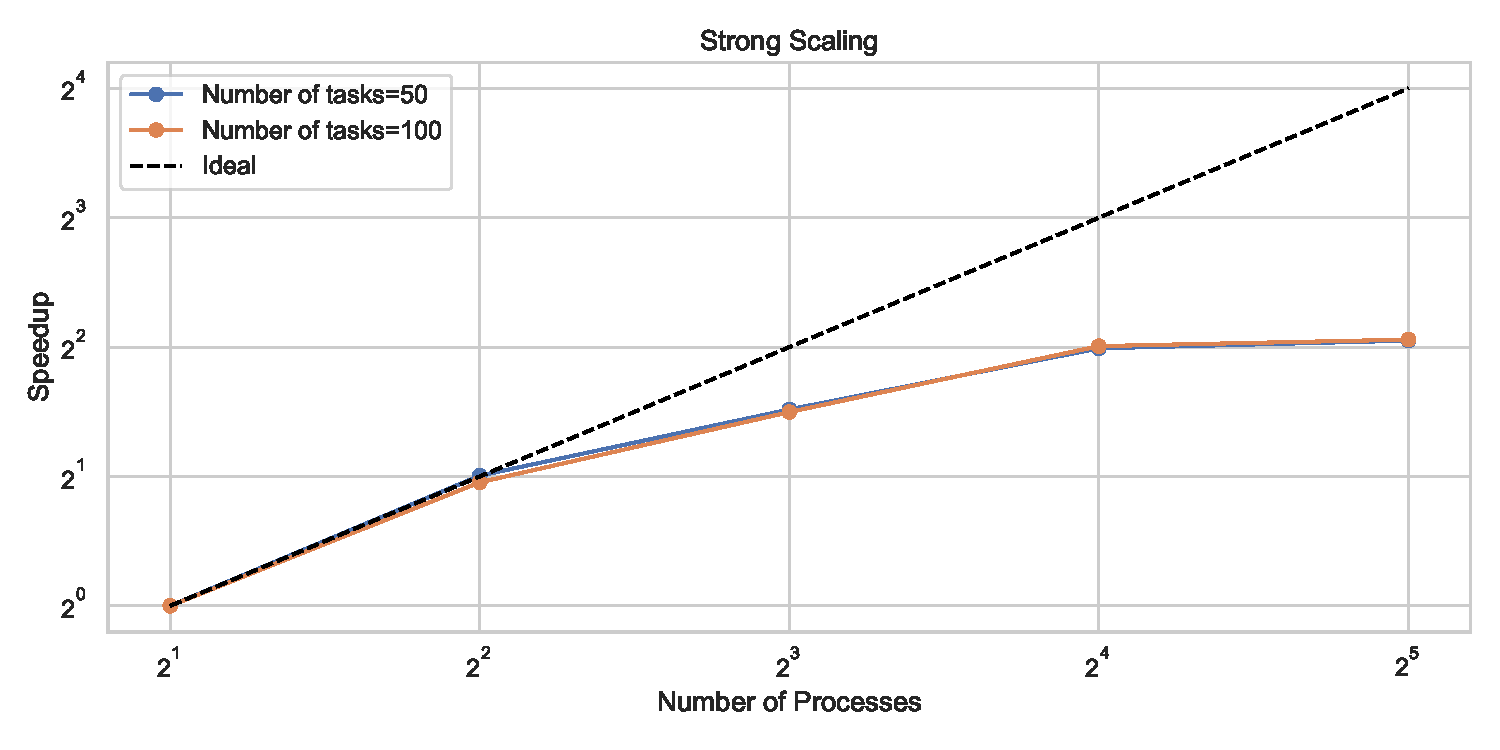
\includegraphics[width=\textwidth]{../hpc_python/ManagerWorker/strong_scaling_plot.pdf}
    \caption{Strong scaling of the parallel Mandelbrot set computation with
    manager-worker implementation on a $4001 \times 4001$ grid with 50 and 100 tasks.}
    \label{fig:mandelbrot}
\end{figure}
The reference was the case of 2 processes (1 worker and 1 manager) and 1 task.
We can see that the speedup is consistent for all both cases of number of tasks,
it is a good result that matches expected behaviour. For a high number of
processes, the speedup declines a bit due to the communication overhead, but
this is expected.
Finally, we plot the bar plot of the number of tasks done by each worker for
each configuration. The results are shown in the Figure \ref{fig:tasks}.
\begin{figure}[h!]
    \centering
    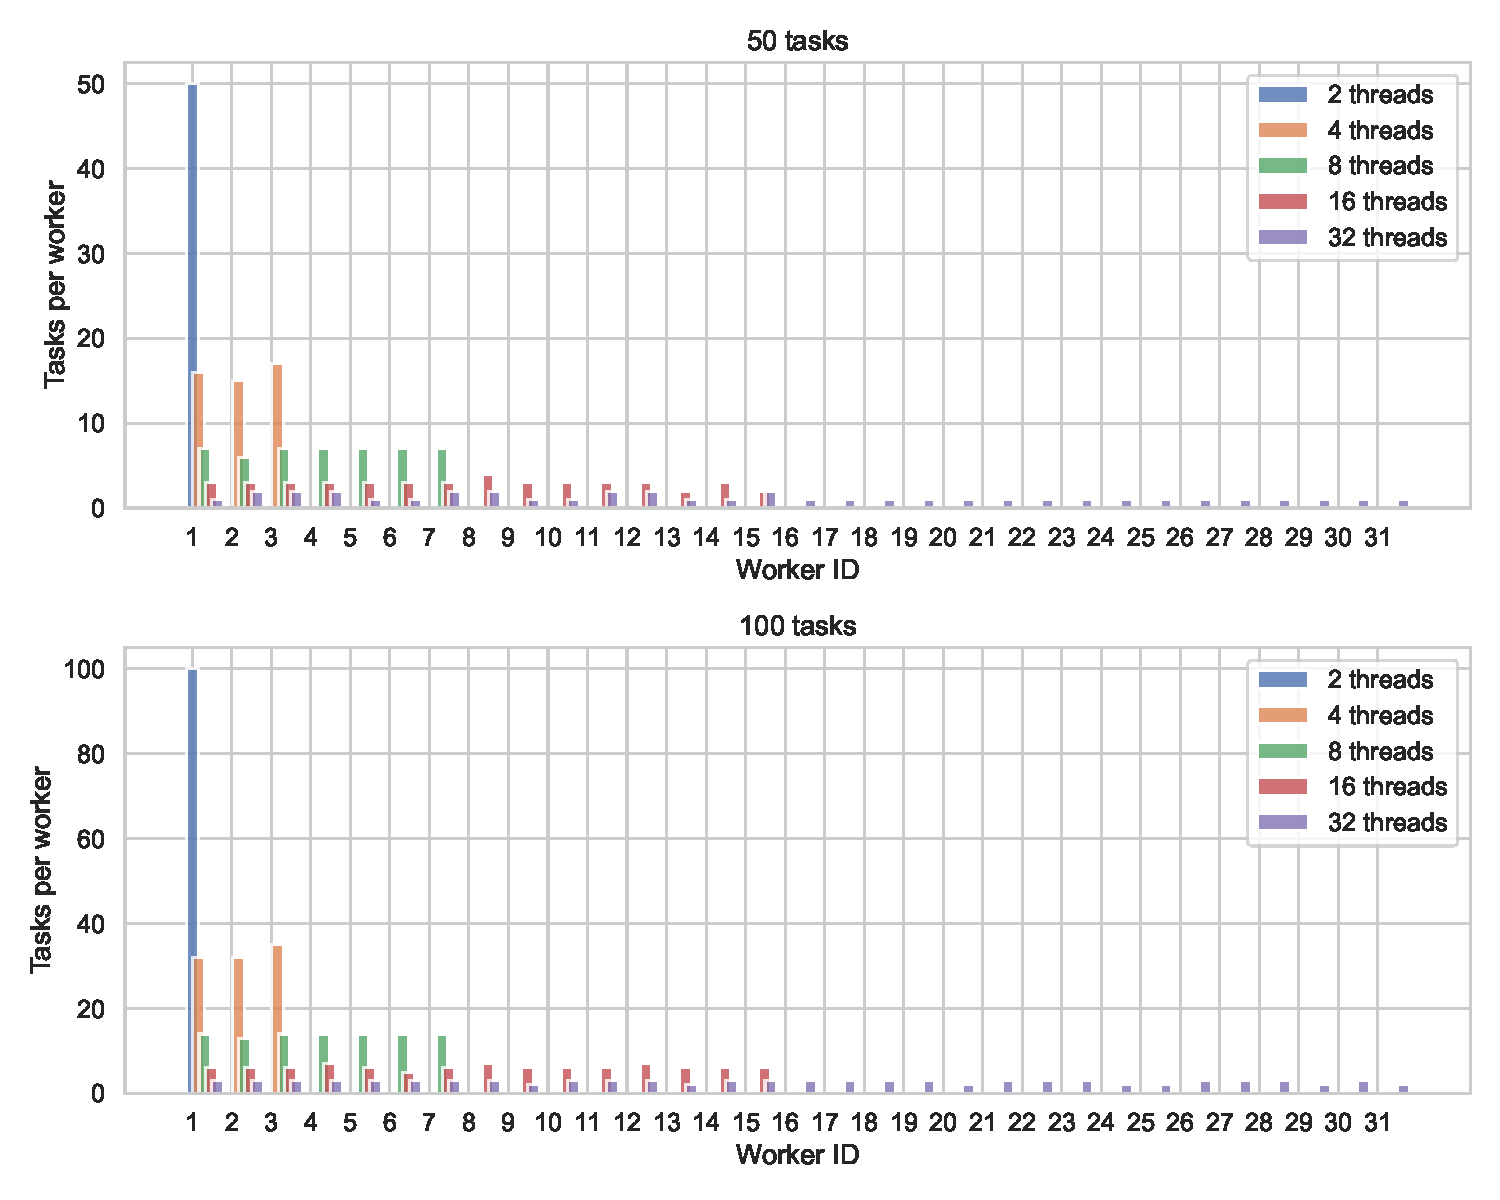
\includegraphics[width=\textwidth]{../hpc_python/ManagerWorker/tasks_per_worker.pdf}
    \caption{Number of tasks done by each worker for each configuration of the
    parallel Mandelbrot set computation with manager-worker implementation.}
    \label{fig:tasks}
\end{figure}
We can see that the number of tasks done by each worker is distributed evenly
for all configurations, which is a good result. This is expected since the
tasks are distributed by the manager as soon as they are completed. For the
plot, I tool the mean of the 50 runs, and that is why they are very even through
the workers, since by the nature of the Mandelbrot set, some regions are more
computationally expensive than others. We can also see that the behaviour is
very similar for 50 and 100 tasks, which is a good indicator of the consistency
of the implementation.
\end{document}
